
% this file is called up by thesis.tex
% content in this file will be fed into the main document

%: ----------------------- introduction file header -----------------------
\chapter{Scalable Creation and Inference of Topics}\label{ch:scalability}

\graphicspath{{scalability/figures/}}

% -------------------------------------------------------------
% -- Scalability
% -------------------------------------------------------------

This chapter presents two essential elements that define the technological environment where our research have been implemented and evaluated. An open and scalable text processing framework is introduced to analyze large document corpora and create probabilistic topic models, and a web-based interface to distribute and reuse those models is proposed. Both the framework and the topic-based services are publicly available to anyone interested in using them.

%This chapter presents \textit{librAIry}\footnote{http://librairy.linkeddata.es}, our text management platform that combines natural language processing techniques with automatic learning algorithms to analyze large collections of documents.  It serves as a technological framework where we can implement the advances of our research and measure its performance. 

\section{Document Workflow}

Given the huge amount of textual data about any domain that is being produced, it becomes crucial to provide mechanisms for efficiently processing this raw data so we can make sense out of it: discarding all the noisy, non-relevant information and keeping only the data that can bring value for an specific purpose. Through computer models created by natural language processing (NLP) methods, these and other more complex tasks can be carried out from text collections\cite{Jurafsky2000SpeechAL}. 

There are multiple tools available that support NLP. While some of them allow for advanced sense-making operations, others opt for composing a solution where different analysis techniques are integrated under a uniform data schema. However, this integration involves significant efforts on reconciling data sources, coordinating processing operations, and efficiently exploiting results from the execution of those techniques. A more flexible paradigm is needed where tools and algorithms for textual document analysis, from different technologies, can operate independently but in a collaborative manner through a common document-oriented workflow. 

%In scientific domain, personalized recommendation of research papers based on their content is a key novel feature for performing a smart selection of relevant resources over very big collections of scientific content. From the set of values and different attributes extracted from the papers and by generating advanced knowledge models about the information they contain we can bridge across the different relevant pieces of information and allow users to navigate them in a more efficient and powerful way. This knowledge about a specific document is frequently acquired by different techniques focused on revealing certain aspects of it, that are later combined to achieve one particular task. 

The architecture presented in this thesis aims to ease the way different algorithms work together and lays the foundation for efficiently process big volumes of textual documents in a distributed and decoupled manner.

\section{librAIry}\label{sec:librairy}

\textit{librAIry} is a framework where different text mining tools, available in various languages and technologies, can operate in a distributed, high-performance and isolated manner creating a common workflow through their actions. Instead to work towards a pre-defined sequence of actions, synchronization across modules is achieved through the aggregation of the operations executed by them in response to an emergent chain of events. This raises both technical and functional challenges to coordinate multiple executions. From the technical point of view, isolated environments and communication mechanisms are provided so initially dissimilar tools can be executed with maximum guarantees. From the functional point of view, all executions are coordinated to reach a final result as aggregation of partial results derived from each execution.

\subsection{Functional Features}
The architecture is articulated around three main concepts: (1) the \textbf{resource} such as \textit{document}, a \textit{part-of-a-document}, or a \textit{domain}. (2) the \textbf{actions} performed over them: \textit{create}, \textit{update} or \textit{delete} a resource. And (3) the new \textbf{state} that is reached by the resource after an action is performed, such as  \textit{created}, \textit{updated} or \textit{deleted}. An \textbf{event} is a message containing details about those three aspects, published on a shared event-bus available for all the modules deployed in the framework. This will, in turn, allow that any module can perform actions on one or more resources in response to a new state reached by a given resource. Actions executed in parallel from distributed environments.

\begin{figure}
  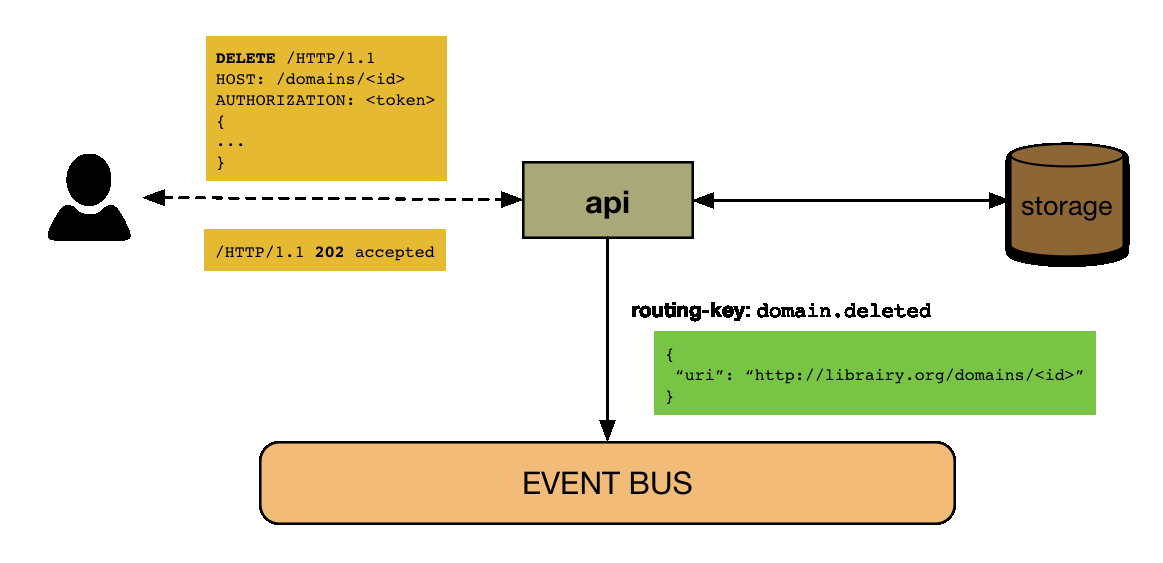
\includegraphics[scale=0.35]{api-domain-deleted}
  \caption{Domain deleted flow.}
  \label{fig:librairy-domain-deleted}
\end{figure}

\subsubsection{Resources}

Two main kinds of resources are considered: those derived from external sources such as (1) \textit{documents} from textual files (e.g. a research paper), (2) \textit{parts} from logical divisions of a \textit{document} (e.g. rhetorical classes or sections), and (3) \textit{domains} from sets of \textit{documents} (e.g. a conference or journal), and those derived from processing the previous ones such as \textit{annotations}. 

To better illustrate this model, consider to explore the research papers published at the SIGGRAPH conference in 2016\footnote{http://s2016.siggraph.org}. First, every paper will be materialized as a new \textit{document} containing the full-text. Immediately after, the \textit{document} will be automatically associated to several \textit{parts}, each of them grouping sentences by rhetorical class (e.g. approach, background, challenge, future work and outcome) and by section (e.g abstract, introduction). Finally, a new \textit{domain} will be created grouping all these \textit{documents}. Different analysis will be performed extending the initial set of resources with more annotations at several representational levels: at \textit{document level}, full-text based annotations are provided such as named-entities, compounds and descriptive tags. At \textit{relational level}, connection between resources are found (e.g. semantic similarity-based relationships). And finally, at \textit{domain level} annotations such as tags and summaries are composed describing the corpus of \textit{documents}.

\subsubsection{Event-based Paradigm}

An event illustrates a performed action, i.e. a resource and its new state. It follows the Representational State Transfer (REST)\cite{Fielding2002} paradigm, but taking into account the state reached after an action, i.e \textit{created}, \textit{deleted} or \textit{updated}. Thus, an event contains the resource type and the new state reached by a specific resource.


\subsubsection{Linked Data Principles }

Data in \textit{librAIry} is individually addressable and linkable \cite{Turchi2012a} following the Linked Data principles defined by T. Berners-Lee \cite{Bizer2009}. Thus, resources (i.e. a \textit{domain}, a \textit{document}, a \textit{part} or an \textit{annotations}) have:
(1) a URI as name, (2) a retrievable (or dereferenceable) HTTP URI so that it can be looked up, (3) a useful information provided by using standard notation (e.g. JavaScript Object Notation (JSON)) when it is  looked up by URI, and (4) links to other URIs so that other resources can be discovered from it.

\subsection{Framework Architecture}

Following a publisher/subscriber approach, all the modules in the framework can publish and read events to notify and to be notified about the state of a resource. 
%For example, when a new \textit{domain} is created, an event-message will be published to the channel: $domain.created$. This event could be managed by one or more modules which will be ready to build models (e.g. a Topic Modeler) by using the \textit{documents} added to that \textit{domain}. 
Therefore, the system flow is not unique and is not explicitly implemented, instead distributed and emergent flows can appear according to particular actions on resources.

\subsubsection{Event-Bus}

We use the Advanced Message Queuing Protocol (AMQP) as the messaging standard in \textit{librAIry} to avoid any cross-platform problem and any dependency to the selected message broker. This protocol defines: \textit{exchanges}, \textit{queues}, \textit{routing-keys} and \textit{binding-keys} to communicate publishers and consumers.A message sent by a publisher to an exchange is tagged with a routing-key. Consumers matching that routing-key with the binding-key used to link the queue to that exchange will receive the message. In \textit{librAIry} this key follows the structure: \textit{resource.status}.Since a wildcard-based definition can be used to set the key, this paradigm allow modules both listening to individual type events (e.g. \'domains.created\' for new domains), or multiple type events (e.g. \#.created for all new resources).

\begin{figure}
  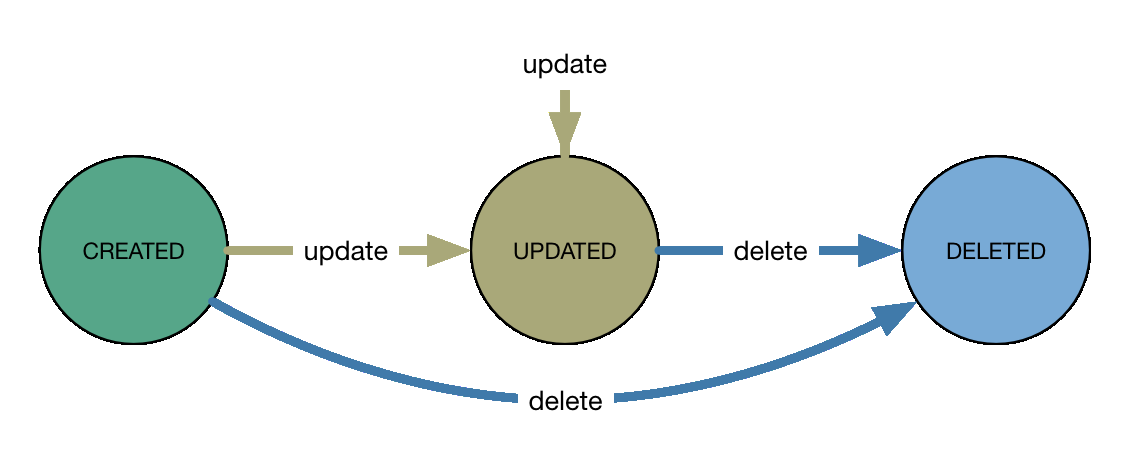
\includegraphics[scale=0.3]{resource-states}
  \caption{Resource states.}
  \label{fig:librairy-states}
\end{figure}

%The \textit{event-message} can not only contain a string of characters in JSON format (default mode), but also an array of bytes serialized in a specific way. 
%The type of the \textit{event-message}, i.e. its routing-key, implicitly defines the format (and serialization) of the message to be understood by both producers and consumers. 

\subsubsection{API}

A HTTP-Rest Application Program Interface (API) was designed for interaction with end-users. Any external operation motivated by a user will be handled here. Some of them, usually those related to reading operations, will be completely managed by this module getting all the data from the internal storage. However, those operations implying a modification of the status of some resource (e.g. creation of a \textit{document}), may be also performed by other modules listening for that type of event asynchronously. This module publishes to the following routing-keys: \textit{domain.(created;updated;deleted)}, \textit{document.(created;updated;deleted)}, \textit{part.(created;updated;deleted)}, and \textit{annotation.(created;updated;deleted)}.

\subsubsection{Storage}

Multiple types of data can be handled in this ecosystem. Inspired in the Data Access Object (DAO) pattern, we have created a Unified Data Manager (UDM) providing access to any type of data used in the system.  Three types of databases have been considered:
\begin{itemize}
	\item \textbf{column-oriented database}: Focused on unique identified and/or \textit{structured data}. This storage allow us searching key elements across resources. 
	\item \textbf{document-oriented database}: Focused on indexing raw text. This storage allow us to execute advanced search operations over all the information gathered about a textual resource. 
    \item \textbf{graph database}: Focused on relations. This storage allow us exploring resources through the relationships between them.
\end{itemize}

\subsubsection{Modules}
The modules composing \textit{librAIry} have been designed following the microservices architectural style. A module is a cohesive (i.e. it implements only functionalities strongly related to the concern that it is meant to model \cite{Dragoni2016}) and independent process working on the framework with a specific purpose. This purpose is defined by both the routing-key and the binding-key associated to the events handled by the module. 

These are the main types of modules identified in \textit{librAIry}:
\begin{itemize}
	\item \textbf{Harvester}: creates system resources such as \textit{documents}, \textit{parts} and \textit{domains}, from local or remote located textual files.
    \begin{itemize}[rightmargin=\dimexpr\linewidth-5cm-\leftmargin\relax]
    	\item Listening for: nothing
		\item Publishing to: \textit{document.(created)}, 
        \textit{part.(created)}, \textit{domain.(created;updated)}
    \end{itemize}
    \item \textbf{Annotator}: retrieves named-entities, compounds, lemmas and other annotations resulting of Natural Language Processing (NLP) task execution from \textit{documents} and \textit{parts}.
    \begin{itemize}[rightmargin=\dimexpr\linewidth-5cm-\leftmargin\relax]
    	\item Listening for: \textit{document.(created;updated)}, \textit{part.(created;updated)}
		\item Publishing to: \textit{annotation.(created;deleted)}
    \end{itemize}
    \item \textbf{Modeler}: builds representational models from a given \textit{domain}. 
    \begin{itemize}[rightmargin=\dimexpr\linewidth-5cm-\leftmargin\relax]
    	\item Listening for: \textit{domain.(created;updated)}
		\item Publishing to: \textit{annotation.(created;deleted)}
    \end{itemize}
\end{itemize}

\begin{figure}
  \includegraphics[scale=0.25]{modules}
  \caption{Modules.}
  \label{fig:librairy-modules}
\end{figure}


\section{Model-as-a-Service}
...

\section{Summary}

In \textit{librAIry}, existing algorithms and tools coming from different technologies can work collaboratively to process and analyze large collections of textual resources which has been successful applied to some real scenarios \footnote{\url{http://drinventor.dia.fi.upm.es}}.
 
A new model definition based on the previously mentioned principle of maximizing information re-usability and minimize irrelevant data is being studied to create a more fine-grained resource design. New domains, in the sense of particular vocabularies or specific textual formats, are also being analyzed to be included into the system via specific harvesters or more precise annotators. Moreover, a template-based mechanism oriented to facilitate the integration of new tools and techniques into the system is being built to make easier to develop new modules as well as increasing the available modules at Docker-Hub.